\chapter{Use cases}
\label{chapter:use cases}
\section{Possible missions}
\subsection{Search and Rescue}

\textbf{Scenario} \newline
A group of tourist are stuck on a snowy side of a mountain where human intervention
is difficult and possibly deathly.
\textbf{Solution} \newline
A 3 drone fleet is dispatched for searching. Each drone is equipped with a different
type of sensor, an infrared camera, a thermal camera and a video camera. Depending
on geography and weather conditions, none of the specified sensors would be able
to guarantee the success of the mission while the fleet has a higher rate of success.
In this situation a \textit{Line Astern Formation} and depending on the sensors
different altitudes may be necessary. For accomplishing the mission the leader
would have programed a flight route and the followers would be guided by it's
actions. If one of the sensors detects a potential survivor the data location
is send to the control centered where a human agent would take into account
the information received from all the sensors and mark the zone for human 
intervention.

\subsection{Mapping}
\textbf{Scenario} \newline
A area needs to be mapped for division in sub-zones for agricultural purposes.
\textbf{Solution} \newline
The zone may have a difficult geography and photographies from different
perspectives would be needed. A fleet of 3 drones with the same type of camera
flying in a \textit{V Formation} would provide sufficient data for a detailed 
analysis to be conducted. The leader would have either a spiral flight path 
or a rectangular flight path to follow. After the entire zone is swept, the data
received from the cameras can be combined to obtain an accurate description
of the interest area.

\section{Surveillance}
\textbf{Scenario} \newline
An traffic accident site has to be supervised and video data has to be live
streamed to a central base.
\textbf{Solution}
An accident site is usually contained to a small zone, being the perfect
candidate for a circular flight path. A situation an object is on fire could
generate problems for a video camera is ideal for a fleet of drones with 
both video and infrared sensors. In this way different information can be 
analyzed and better decisions can be made for resolving the situation.

\section{Evaluation and Results}
The approach proposed in this thesis was tested using the architecture described in
\labelindexref{Chapter}{chapter:uav-management-framework}. Each UAV was simulated
using a dedicated FGFS instance connected to an FGMS instance. The centralized
data was collect for display using QGC and for manipulation the CAN Simulator
developed for the Autonomous UAV project.

The leader had it's own defined path where his heading was changed to steer in
a predefined direction. The simulations ran included tests were the leader
was flying in a straight line or where is changed it's direction by up to 
$90^{\circ}$. The test had the role to observe the drones ability to follow
the leader,  the stability of the formation and also the percentage of time
that each UAV spent in the \textit{Synchronization Mode} or \textit{Formation Maintaining
  Mode}
  

The Line astern formation was tested using 3 drones with two scenarios. In 
the first scenarios the followers were supposed to flight at the same altitude
as the leader. In the second scenarios the airplanes had different altitude offsets
ranging between -40 and 40 feet. Another test scenario that was tested was 
a V Formation.

During the simulations it has been observed that a delay in communication 
can lead to a formation loss that sets the drones in the \textit{Synchronization Mode}.
The effects in the communication delay can be seen in \labelindexref{Figure}{img:delay-1}
and \labelindexref{Figure}{img:delay-2}.

\fig[scale=0.5]{src/img/delay-1.png}{img:delay-1}{Delay influence part. I .}

\fig[scale=0.5]{src/img/delay-2.png}{img:delay-2}{Delay influence part. II .}
\newpage
In \labelindexref{Figure}{img:delay-1} the effects of the communication delay
is mild and it can be observed at crossbars A and D. At cross bar it can
be seen that the green UAV receives data about the leader that correspond to 
about 3 seconds back in time. The computation error induces a heading that is 
with $4^{\circ}$ smaller that the leaders heading. The maximum distance reported
by FGMS between the leader (read UAV) and the green UAV is 729 feet. The formation
range was set to be between 300 and 500 feet. According to this the read UAV
steers right starting at crossbar C. Near crossbar D it can be observed that 
the red UAV stabilizes and uses the same heading as the leader. From the point
of view of the violet UAV, there delay can be observed near crossbar D, when
the reported distance to the leader is 778 feet. The error detected at crossbar 
D is quickly corrected, the UAV steering right and stabilizing near the leader.
In the same figure it than be also be observed that the module has stopped reporting
heading because of the collision avoidance necessity. It can be clearly observed
that at point A the green UAV steers left, but the violet one maintains the
same heading as the leader. The distance between the leader and the violet UAV
in point A was reported to be 286 feet, lower that the accepted 300 feet threshold.
At that moment the collision avoidance should assume control. When the violet UAV
reaches point B,  the leader is reaches crossbar B' having a distance of 450 feet, 
thus determining the drone to move towards the designated position in formation.

In \labelindexref{Figure}{img:delay-2} the delay has a more prominent effect.
At crossbar A it can be seen how the green UAV receives data that correspond
with the start of the flight path, having a heading of $45^{\circ}$. Until the
correct data is received the distance from the leader is increased to approximately
2300 feet. At crossbar B the green drone adopts a heading that allows it to fly
towards the correct position. As in \labelindexref{Figure}{img:delay-1} 
it can be observed that the violet drone considers the distance small enough
to give control to the \textit{collision avoidance} module,  assuming
the correct position after crossbar D.

From the simulation that generated the flight path visible in 
\labelindexref{Figure}{img:delay-1} the UAVs have used flight modes with the 
time percentages visible in \labelindexref{Figure}{img:flight-modes}. The
\textit{Unattended mode} is represented by the program start-up when the 
drone are flying only with the initial startup parameters. The \textit{Unattended mode}
is used until the first message from the \textit{Formation Flight} mode is received.
The collision avoidance time is measured as the time as the \textit{Formation
Flight Module} reports the same heading for a distance below the minimum accepted
limit.

\fig[scale=0.4]{src/img/flight-modes.png}{img:flight-modes}{Time percentage of
flight modes usages.}

Using FGMS to display all the drones in the same environment for a \textit{Line
  Aster} formation  \labelindexref{Figure}{img:line2} and \labelindexref{Figure}{img:line1}
were captured during the simulations. In the simulation for \labelindexref{Figure}{img:line2}
the computational error introduced a lateral distance varying from 6 to 10 which
is considered to be an acceptable error. In both simulation the leader was
climbing constantly with a rate of $3feet/s$.

\begin{figure}[p]
\centering
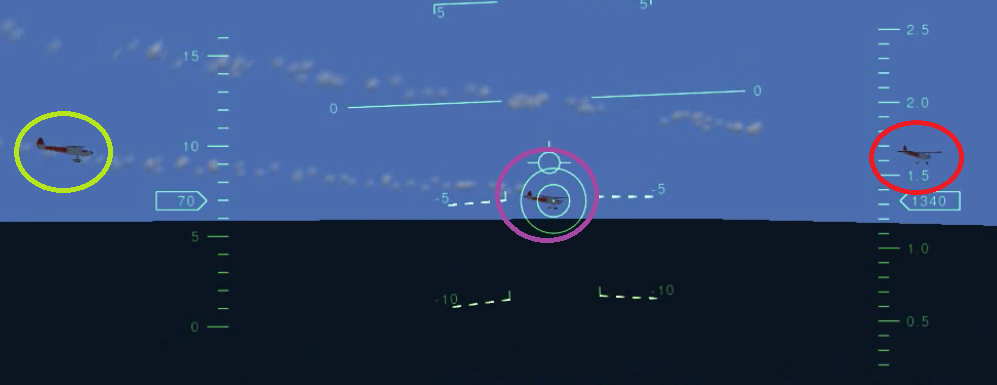
\includegraphics[scale=0.5]{src/img/line2.png}
\label{img:line2}
\caption{Line Astern with same elevation.}
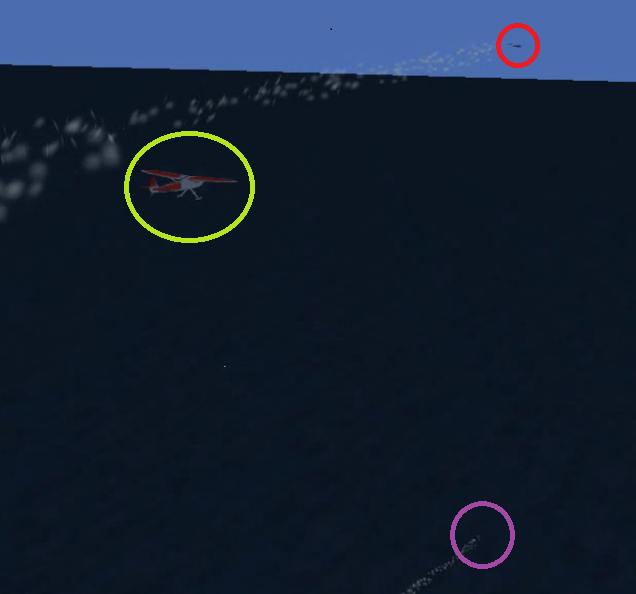
\includegraphics[scale=0.8]{src/img/line1.png}
\caption{Line Astern with elevation difference.}
\label{img:line1}
\end{figure}
\newpage

A successful formation flight simulation can be seen in \labelindexref{Figure}{img:lineqgc}.
In this figure it can be seen that that the line formation needs a special stabilization
mechanism for determining when the drone is on the same flight path as the leader.
Although \labelindexref{Equation}{eqn:side-of-line} states that a point
is on the desired line if the the $sign$ is equal to 0, computational error
makes impossible to use this formula for perfect alignment. 
\fig[scale=0.7]{src/img/lineqgc.png}{img:lineqgc}{Line Astern Flight Path}. 

Compared to the \textit{Line Astern Formation} the \textit{V Formation} stabilizes 
perfectly from the point of view of the heading. Once the UAV moves to the 
correct side of the leader, it only adapts the distance until it reaches a value
that is in the predefine range predefined of accepted distances. For example
\labelindexref{Figure}{img:vqgc} presents the forming and maintaining of a V
Formation. In this simulation it is also observed that there are no communication
delays introduces, thus being an ideal simulation.
\fig[scale=0.7]{src/img/vqgc.png}{img:vqgc}{V Formation Flight Path}. 
\newpage
The possible cause for the communication delay could be introduced by the 
congestions from the network or by the intense computation executed by the FGFS
instances needed to render all the UAVs in the same environment while communicating
with different external modules.
% % \todo {captures of 3 formations}
% \todo {captures of flight-path}


